% !TeX spellcheck = en_US
\documentclass[letterpaper,12pt,twoside]{report}
\usepackage{fancyhdr}
\usepackage{fullpage}
\usepackage{tikz}
\usepackage{amsmath}

\begin{document}
	\pagestyle{fancy}
	\fancyhf{}
	\fancyhead[L]{Day 26}
	\fancyhead[R]{\textit{The Calendar Project}}
	\fancyfoot[L]{Citations Involved: ???}
	
	% Problem
	\paragraph{Problem}
	\begin{quote}
		\textsf{In equilateral triangles $ABC$ and
			$ADE$, $AB=3$  in and $BD = \dfrac{AB}{3}$  in. Find
			the area of the shaded triangle $CDF$.}
	\end{quote}
	
	% Graphics
	\begin{center}
		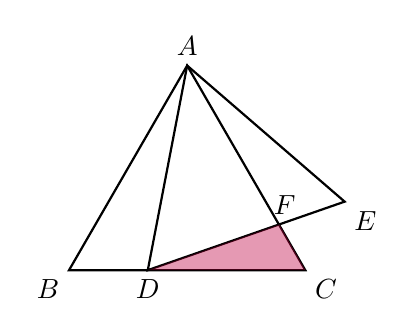
\begin{tikzpicture}
		\draw[thick] (0,0) -- (3,0) -- (1.5,2.598) -- cycle;
		\draw[thick] (1,0) -- (3.5,0.87) -- (1.5,2.598) -- cycle;
		
		\node[above] at (1.5,2.598) {$A$};
		\node[below left] at (0,0) {$B$};
		\node[below right] at (3,0) {$C$};
		\node[below] at (1,0) {$D$};
		\node[below right] at (3.5,0.87) {$E$};
		\node[above] at (2.74,0.58) {$F$};
		
		\draw[fill=purple,opacity=0.4] (3,0) -- (1,0) -- (2.67,0.58);
		\end{tikzpicture}
	\end{center}
	
	% Reasoning
	\paragraph{Reasoning}
	\begin{quotation}
		
		???
		
	\end{quotation}
	
	\paragraph{External References}
	
	\begin{enumerate}
		\item ???
	\end{enumerate}
	
\end{document}